\documentclass[11pt]{amsart}
\usepackage{geometry}                % See geometry.pdf to learn the layout options. There are lots.
\geometry{letterpaper}                   % ... or a4paper or a5paper or ... 
%\geometry{landscape}                % Activate for for rotated page geometry
%\usepackage[parfill]{parskip}    % Activate to begin paragraphs with an empty line rather than an indent
\usepackage{graphicx}
\usepackage{amssymb}
\usepackage{epstopdf}
\DeclareGraphicsRule{.tif}{png}{.png}{`convert #1 `dirname #1`/`basename #1 .tif`.png}

\title{Brief Article}
\author{The Author}
%\date{}                                           % Activate to display a given date or no date

\begin{document}
%\maketitle
%\section{}
%\subsection{}


In [Weissman, Illustrated Theory of Numbers (AMS)], there is a nice description of how to generate a mapping between reduced fractions and pythagorean triples.

In outline the method is as follows:

Take the unit circle $x^2+y^2=1$ and a straight line through $(0,1)$ with a rational gradient $m$, i.e. $y = mx + 1$ (see picture).

The the line  and the circle intersect at $(0,1)$ and $(u,v)$. The coordinates can be found to be 
$$
u = -\frac{2 m}{{{m}^{2}}+1} \qquad 
\text{ and }
\qquad
v = -\frac{{{m}^{2}}-1}{{{m}^{2}}+1}
$$

As $m$ is rational, we can write it as $a/b$ with gcd$(a,b)=1$ and we can re-write $u$ and $v$.
$$
u = =-\frac{2 a b}{{{b}^{2}}+{{a}^{2}}}
\qquad 
\text{ and }
\qquad
v = =\frac{{{b}^{2}}-{{a}^{2}}}{{{b}^{2}}+{{a}^{2}}}
$$

Using the fact that $u^2+v^2 = 1$ leads to
$$
(2ab)^2 + (b^2-a^2)^2 = (b^2 + a^2)^2
$$
which gives a pythagorean triple $2ab$, $b^2-a^2$ and $a^2+b^2$ for which it is possible to show that only 1 is a common divisor.

Later on, there is an exercise to show that XXXXX

The hint is to use the point $(1,1)$ instead of the point $(0,1)$ in a similar argument to that given above.

When I do this, I get quite complex expressions for the intersection coordinates.

\newpage

\begin{center}
\includegraphics{pics/pythag-triples}
\end{center}





































\end{document}  